\documentclass{article}
\usepackage[a4paper, left=1cm, right=1cm, top=1cm, bottom=1cm]{geometry}
\usepackage{graphicx}
\usepackage{pdflscape}
\usepackage{float}

\graphicspath{{img}}

\title{\vspace{4cm}\Huge{Profiling the calculator} \\ \vspace{1cm} \LARGE{Output of the profiler}\vfill}
\author{Patrik Skaloš, xskalo01 \vspace{5cm}}
\date{}

\begin{document}

  \begin{landscape}

    \maketitle

    \begin{center}

      \Large{Output of the profiler when calculating the standard deviation of \textbf{10} numbers within range \textless 0, 1000000\textgreater}\\
      \vspace{1cm}
      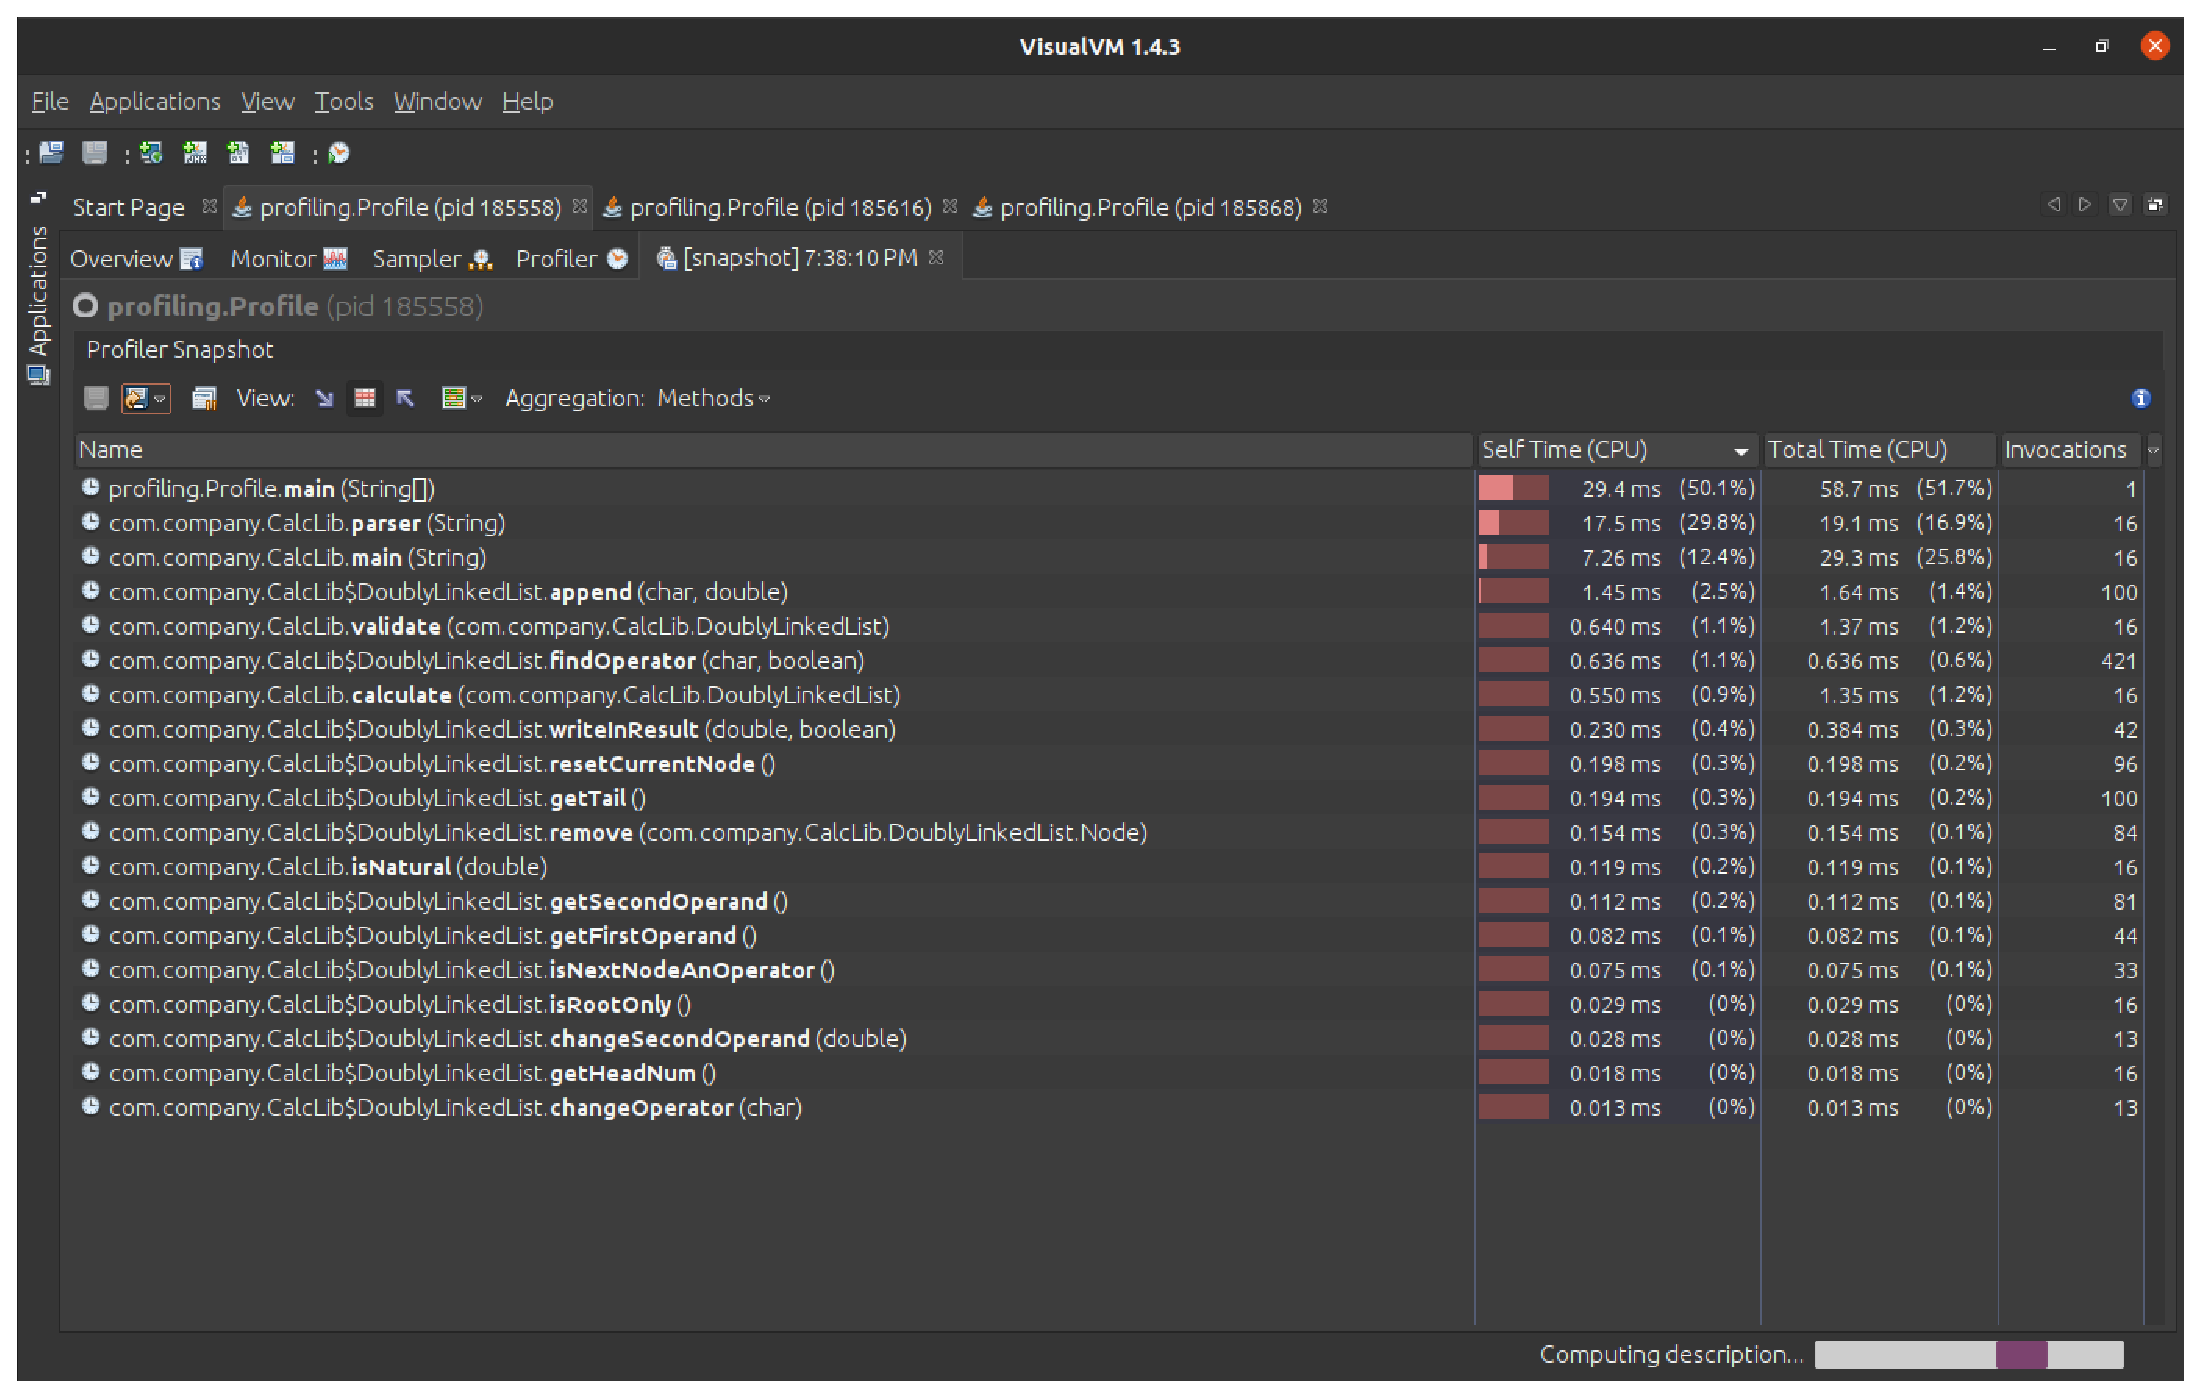
\includegraphics[width=26cm]{profiling_result-10_numbers.eps}

      \newpage

      \Large{Output of the profiler when calculating the standard deviation of \textbf{100} numbers within range \textless 0, 1000000\textgreater}\\
      \vspace{1cm}
      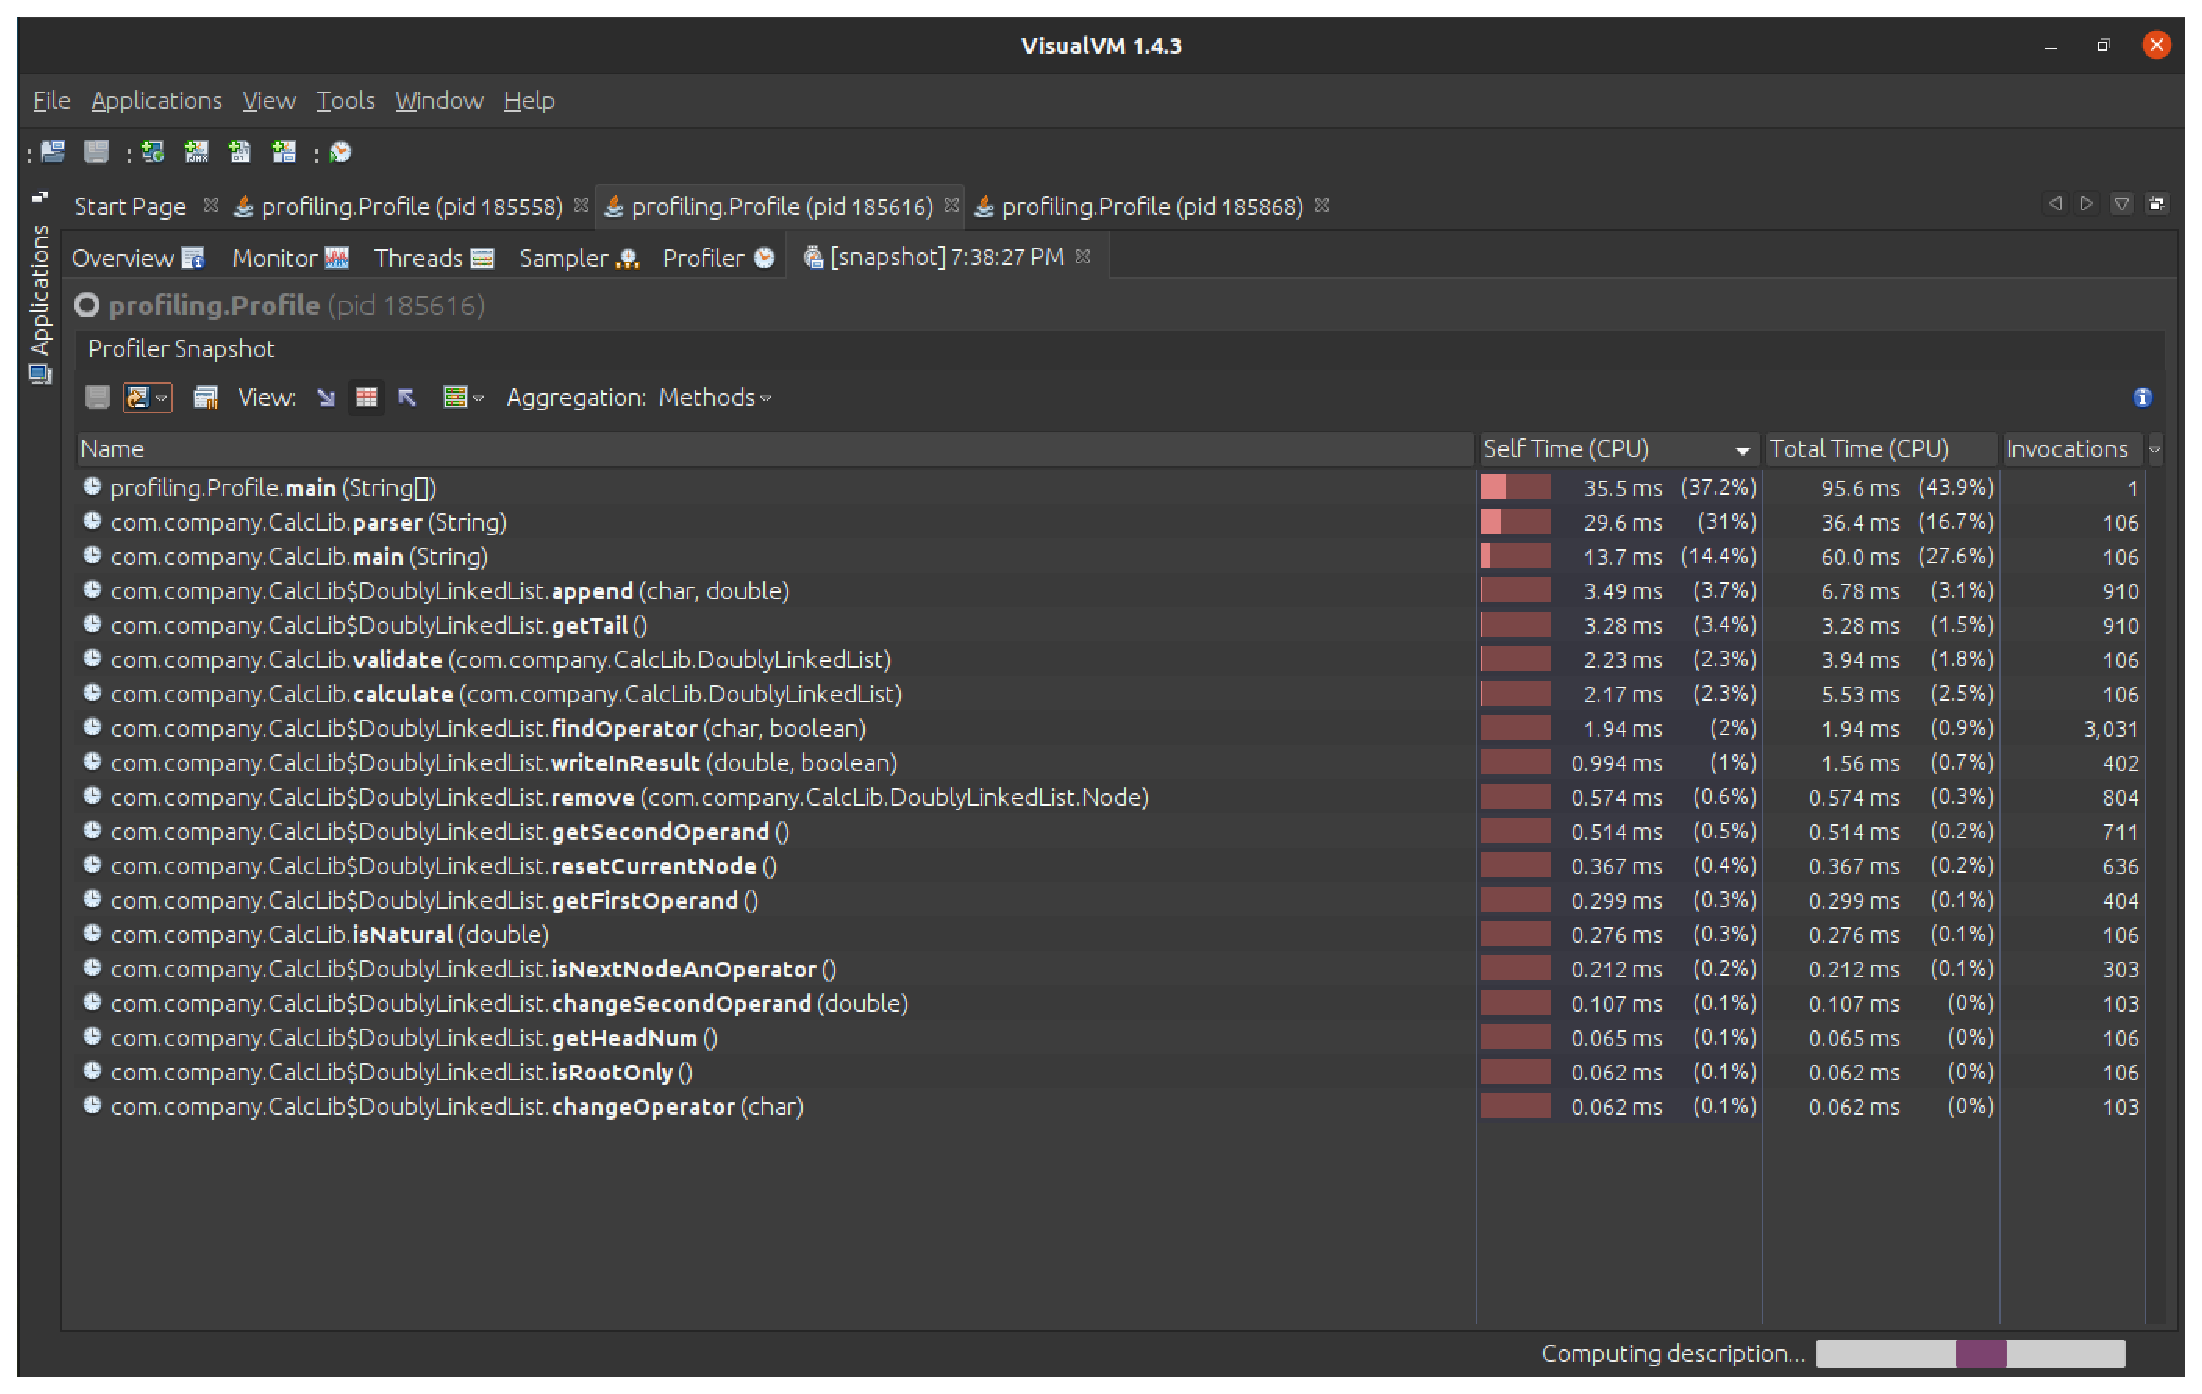
\includegraphics[width=26cm]{profiling_result-100_numbers.eps}

      \newpage

      \Large{Output of the profiler when calculating the standard deviation of \textbf{1 000} numbers within range \textless 0, 1000000\textgreater}\\
      \vspace{1cm}
      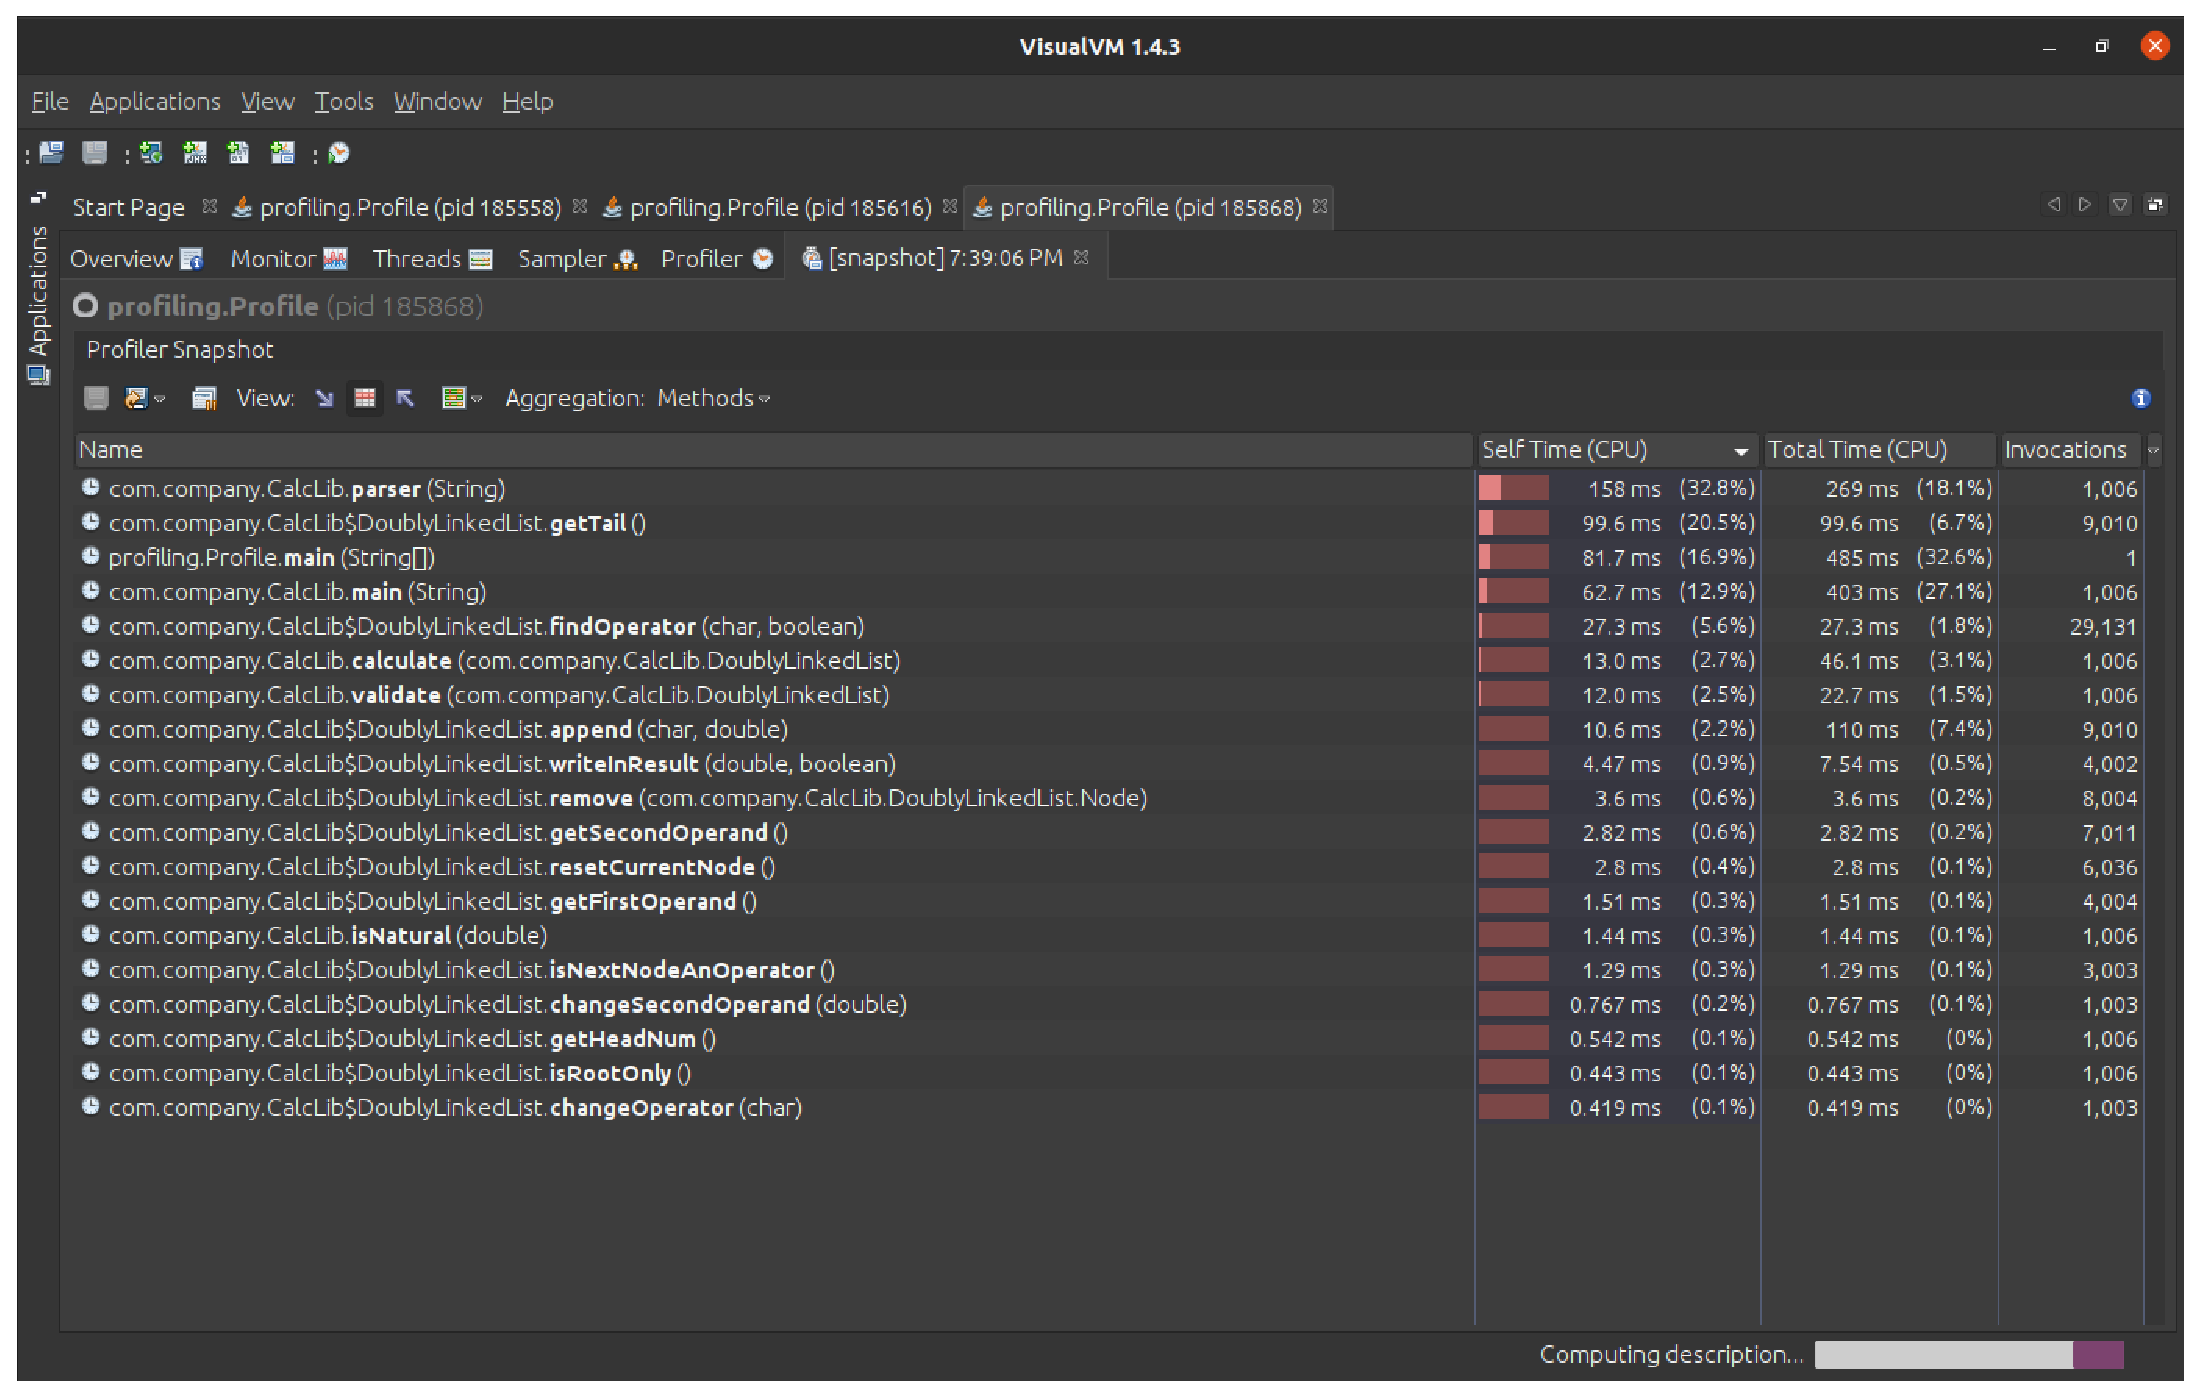
\includegraphics[width=26cm]{profiling_result-1000_numbers.eps}

      \newpage

      \Large{Output of the profiler when calculating the standard deviation of \textbf{10 000} numbers within range \textless 0, 1000000\textgreater}\\
      \vspace{1cm}
      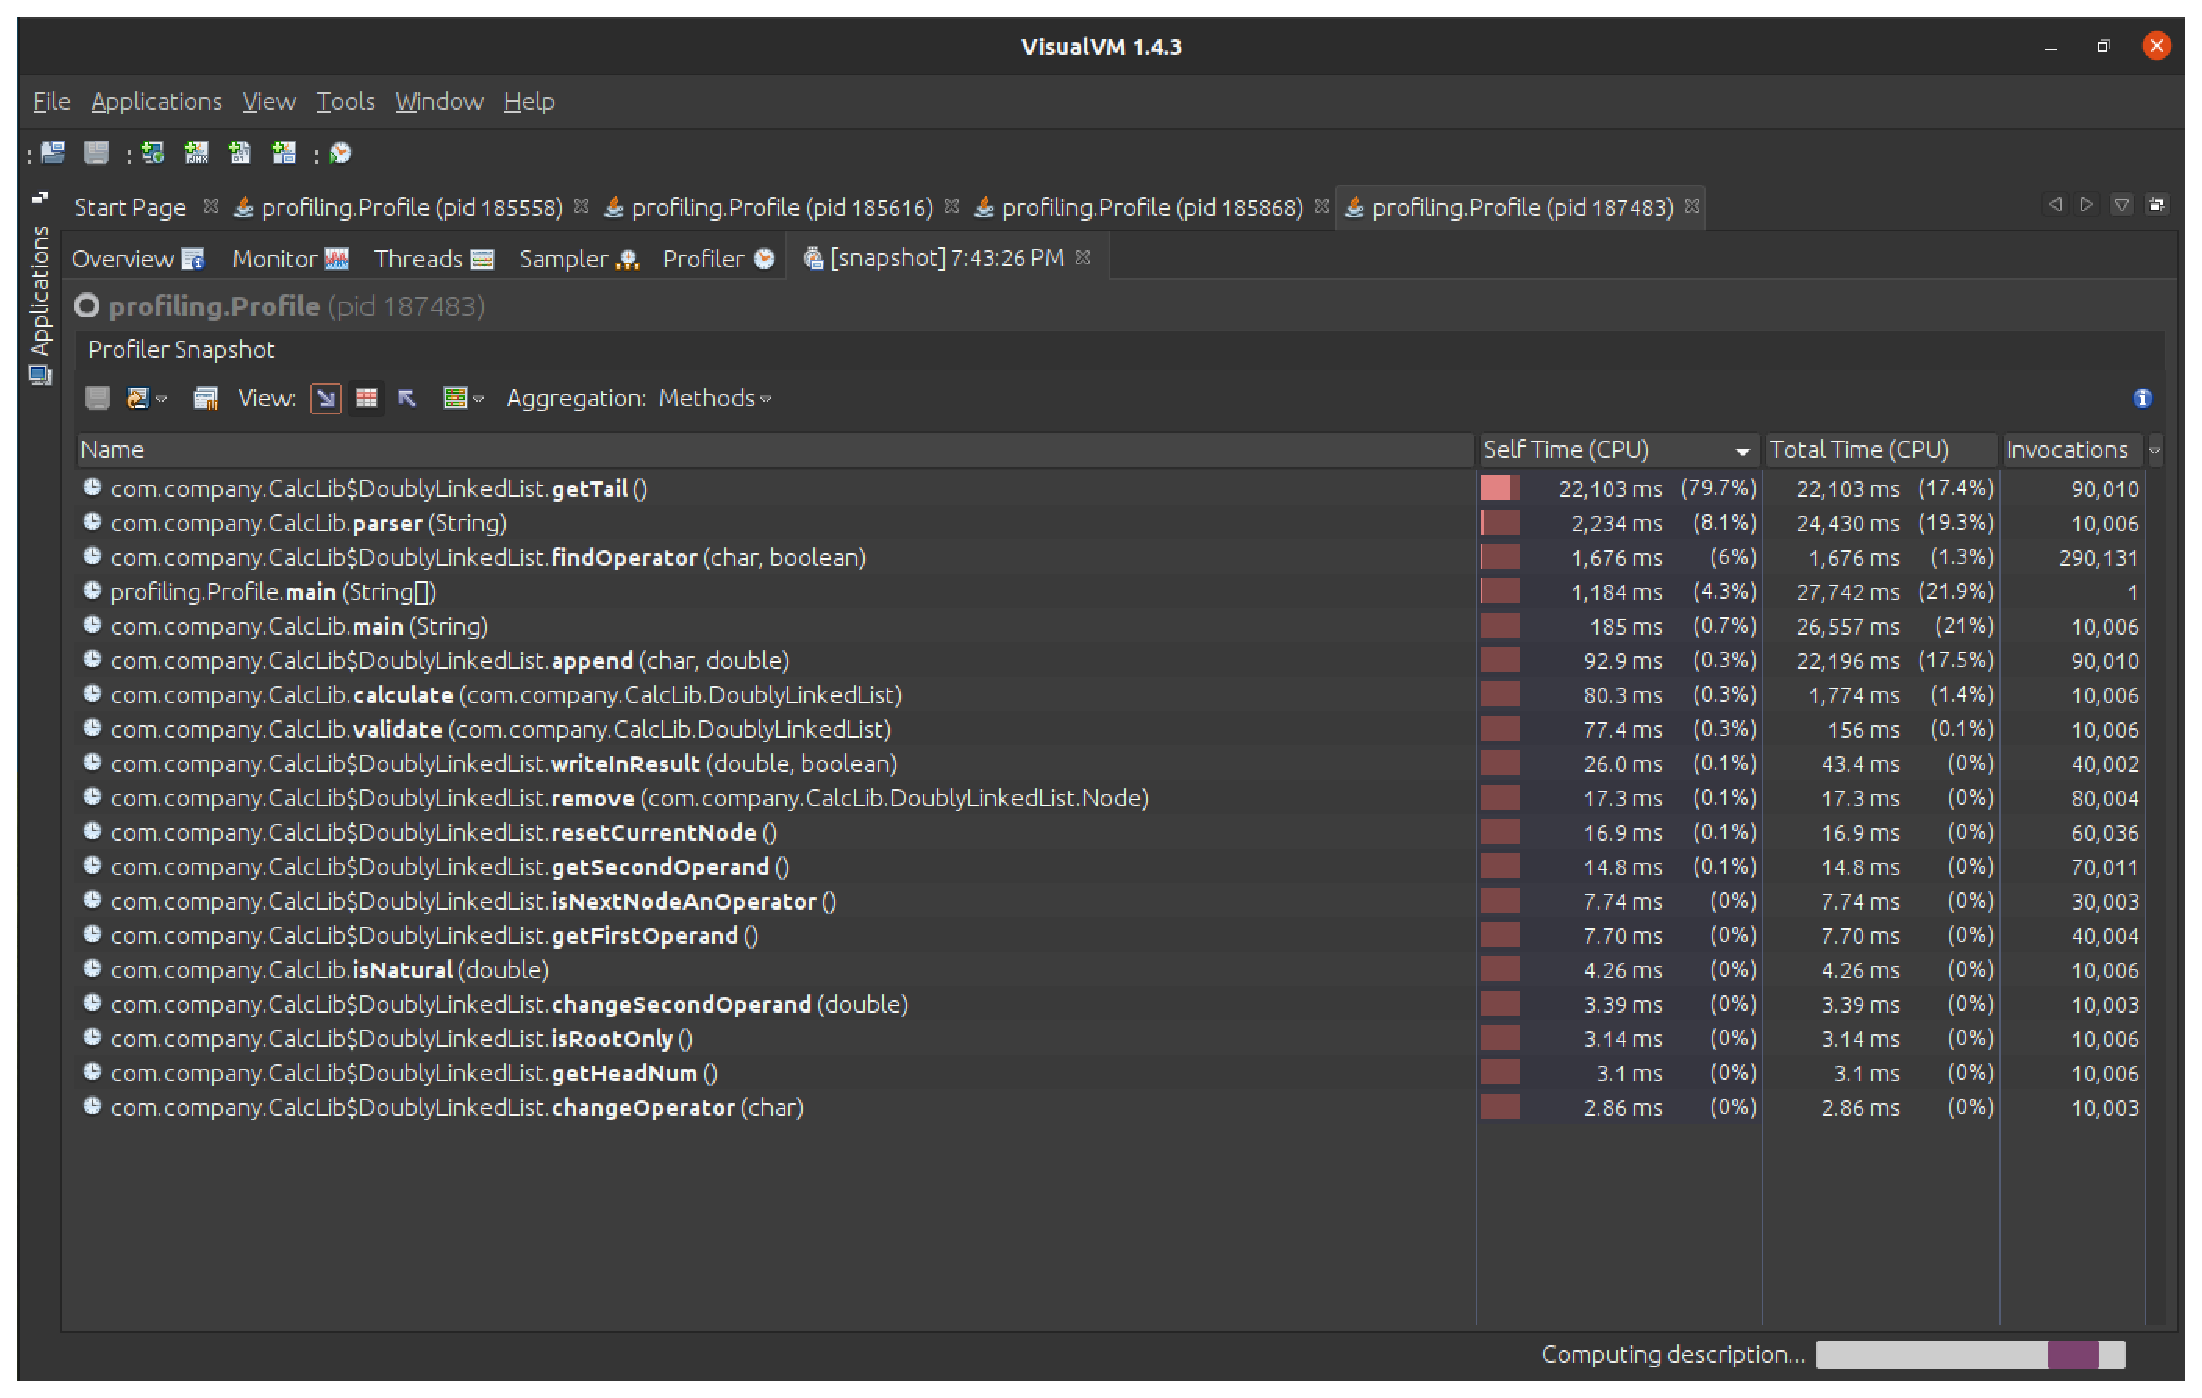
\includegraphics[width=26cm]{profiling_result-10000_numbers.eps}

    \end{center}
  \end{landscape}

\end{document}
